\section{Measuring parametrization effects}
\label{sec:parametrizing}

After implementing the \ac{pimc} search previously described, some tests were executed in order to observe the effects of different parametrizations.
However, these tests had to be comparative and a baseline or benchmark was required to establish a standard measure.


\subsection{Creating benchmarks}
The baseline agent was called Rule-based and its main idea was to chose a move considering predefined rules, instead of using hard computational algorithms.
The following pseudo-code illustrates the deliberation process of this agent and tries to roughly reproduce the reasoning of a non-professional human player.

\begin{algorithm}
	\caption{Rule-based Sueca algorithm}
	\begin{algorithmic}[1]
		\Procedure{RuleBasedDecision}{InfoSet $I$}
			\State $HighestCardPerSuit$ = GetHighestCardPerSuitFromHand($I$)
			\ForAll {$h \in HighestCardPerSuit$}
				\If{isHighestUnplayedFromSuit($h$)}
					\If{GetSuit($h$) = TRUMP \&\& CountCardsFromSuit($I$) > 5}
						\State \textbf{return} h
					\ElsIf{GetSuit($h$) $\not=$ TRUMP \&\& CountCardsFromSuit($I$) > 5}
						\State \textbf{break}
					\ElsIf{GetSuit($h$) $\not=$ TRUMP}
						\State \textbf{return} h
					\EndIf
				\EndIf
			\EndFor
			\State \textbf{return} GetLowestCardFromHand($I$)
		\EndProcedure
	\end{algorithmic}
	\label{alg:pimc}
\end{algorithm}

It starts by collecting the highest cards of each allowed suit for the current play.
The possibility of playing such a highest card is granted by two requirements: being the highest unplayed card of that suit; and not holding at least other 5 cards from that suit, except for the trump suit.
Otherwise, this rule-based player return the lowest possible card.

The first experiments to test this baseline player compare three different scenarios:
\begin{itemize}
\item (a) 1000 games with 4 Rule-based players;
\item (b) 1000 games with 1 Rule-based player and 3 Random players;
\item (c) 1000 games with 2 Rule-based players against 2 Random players.
\end{itemize}

\begin{figure}[h]
        \centering
        \begin{subfigure}[h]{0.32\textwidth}
                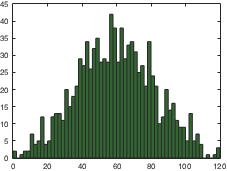
\includegraphics[width=\textwidth]{./img/5/HA-4RuleBased}
                \caption{Scenario A}
                \label{fig:histogramA}
        \end{subfigure}
        \begin{subfigure}[h]{0.32\textwidth}
                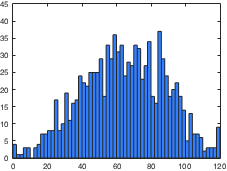
\includegraphics[width=\textwidth]{./img/5/HB-1RuleBased_3Random}
                \caption{Scenario B}
                \label{fig:histogramB}
        \end{subfigure}
        \begin{subfigure}[h]{0.32\textwidth}
                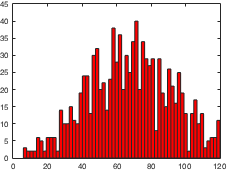
\includegraphics[width=\textwidth]{./img/5/HC-2RuleBased_2Random}
                \caption{Scenario C}
                \label{fig:histogramC}
        \end{subfigure}
        \caption[Histograms of the final points obtained in the 3 scenarios]{Histograms of the final points obtained in 1000 games by: (a) one of the teams; (b) the team with 1 Rule-based player and 1 Random player; (c) the team with 2 Rule-based players}
        \label{fig:histograms}
\end{figure}

The histograms presented on Figure~\ref{fig:histograms} exhibit the distribution of final points in 1000 games by one of the teams in each scenario.
However, comparing the three histograms gets easier when merging the three fitting curves in one graph, Figure~\ref{fig:fitHistABC}.

\begin{figure}[h!]
  \centering
    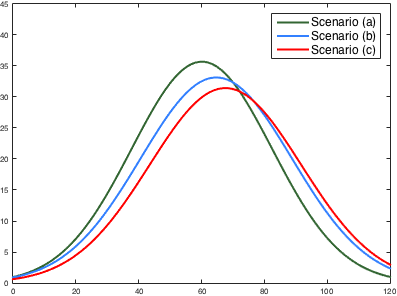
\includegraphics[width=0.5\textwidth]{./img/5/FitHistABC}
  \caption{Fitting curves of histograms presented on Figure~\ref{fig:histograms} with the same colour scheme}
\label{fig:fitHistABC}
\end{figure}

In scenario (a), results were very balanced, as expected, because all players had the same deliberation process.
In 1000 games one of the teams obtained a winning percentage of 48.5\%, a drawing percentage of 1.9\% and a losing percentage of 49.6\%.
The scenario (b) showed that a team with 1 Rule-based player and 1 Random player can beat a 2 Random players team with a winning percentage of 5.6\%, a drawing percentage of 1.8\% and a losing percentage of 41.6\%.
Finally, in scenario (c), the team with 2 Rule-based players beat the the 2 Random players with the highest winning percentage of 61.1\%, a drawing percentage of 1.8\% and losing percentage of 37.1\%.

A player's performance can only be measured when playing with different players, otherwise, playing a considerable amount of games will balance the winning and losing rates, as seen in scenario (a).
Additionally, theses results also demonstrated the impact of the team player on the team score, since having 2 Rule-based players in the same team increased the winning rate of the team with only 1 Rule-based player.

In addition to these conclusions, the winning rates achieved by 1 Rule-based (scenario (b)) and 2 Rule-based (scenario (c)) were lower than expected, since their opponents have completely random procedures for playing the game.
A possible reason might be \emph{Sueca}'s element of chance, which means certain hands can limit the result even though the opponents are Random players.

This idea incited some research on the influence of the players' initial conditions on the game result.
On one hand, the power of a hand is completely dependent on the playing manner of each player, and therefore, using Random players to measure this property is inappropriate.
On the other hand, this measure will not be used to carefully predict a hand's effect on the final result.
Instead, its goal is to generally classify a hand in one out of three distinct categories (\emph{hard}, \emph{medium} and \emph{easy}) and to filter the hands that are hardly or easily capable of winning.
As a result, the chosen scenario to extract these categories' features was (a).

In order to derive such characteristics, the first step is to presume and collect possible features of the initial game conditions that may influence the final result.
After that, computing a linear regression on that data to decide the relevant features.
In the first iterations of this process, many variables were tested for one player of the team and also for both.
For instance, the total points, the trump points, the number of aces, the number of sevens, the number of trumps, being the first to play, having the trump ace, the number of suits.
However, many of them were rejected by the null hypothesis with a significance level of 0.05, and the remaining features were only three: team aces number, team sevens number and team trumps number.

\begin{figure}[h!]
  \centering
    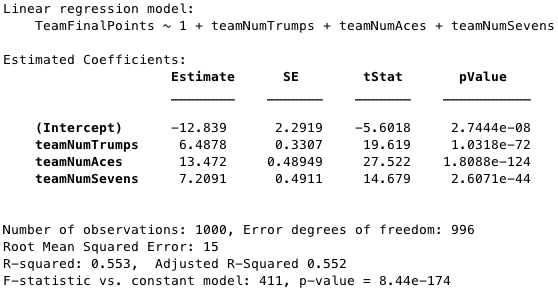
\includegraphics[width=0.7\textwidth]{./img/5/linearRegression}
  \caption{Linear regression with the \emph{team aces number}, the \emph{team sevens number} and the \emph{team trumps number} as predictor variables and \emph{team final points} as the response variable}
\label{fig:linearRegression}
\end{figure}

Figure~\ref{fig:linearRegression} shows the detailed statistic relationship of the mentioned variables on the team final result.
Although the model has a low r-squared value, the p-values of the predictors can reject their null hypothesis and prove their importance in the final result.

\begin{figure}[h]
        \centering
        \begin{subfigure}[h]{0.32\textwidth}
                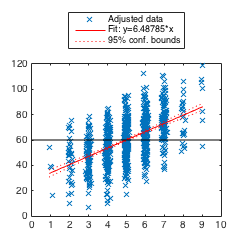
\includegraphics[width=\textwidth]{./img/5/teamTrumpsNumber}
                \caption{Variable \emph{team trumps number}}
                \label{fig:teamTrumpsNumber}
        \end{subfigure}
        \begin{subfigure}[h]{0.32\textwidth}
                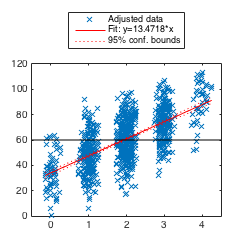
\includegraphics[width=\textwidth]{./img/5/teamAcesNumber}
                \caption{Variable \emph{team aces number}}
                \label{fig:teamAcesNumber}
        \end{subfigure}
        \begin{subfigure}[h]{0.32\textwidth}
                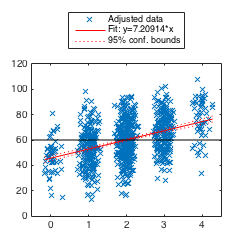
\includegraphics[width=\textwidth]{./img/5/teamSevensNumber}
                \caption{Variable \emph{team sevens number}}
                \label{fig:teamSevensNumber}
        \end{subfigure}
        \caption{Fitting function for each individual predictor variable}
        \label{fig:fitFunctions}
\end{figure}

Finally, Figure~\ref{fig:fitFunctions} can help to quantify the importance of each feature and to build the domain values for each class (\emph{hard}, \emph{medium} and \emph{low}).
Regarding the Figure~\ref{fig:teamTrumpsNumber}, the numbers of initial trumps held by a team, where at least 60\% of the samples were lost games, are 1, 2, 3 and 4..
In the same way, the numbers of initial trumps held by a team, where ate least 60\% of the samples were won games, are 6, 7, 8 and 9.
Applying the same procedure to the three predictor variables, the decided \emph{hard} initial conditions to a team (with low probability of winning) are to have at most 4 trumps, at most 1 ace and at most 1 seven.
Conversely, the decided \emph{easy} initial conditions to a team (with high probability of winning) are to have at least 6 trumps, at least 3 ace and at least 3 seven.
Other cases are considered as \emph{medium} hands.

\begin{figure}[h!]
  \centering
    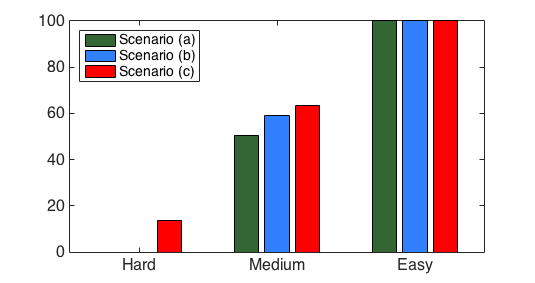
\includegraphics[width=0.7\textwidth]{./img/5/classifiedPercentages}
  \caption{Favourable games percentages grouped by initial hands categorization}
\label{fig:classifiedPercentages}
\end{figure}

On top of the developed classification, the new benchmark for evaluating the \ac{pimc} algorithm is the favourable games percentage (in which the team drew or won) for the three types of initial hands.
As shown in Figure~\ref{fig:classifiedPercentages}, three conclusions can be observed: \emph{easy} initial hands led to won or drew games 100\% of the times in every scenario; the only scenario with the favourable games percentage higher than 0\% with \emph{hard} initial hands was (c); and obtained favourable games percentage in scenarios (a), (b) and (c) were 50.6\% 59.0\% 63.5\%, respectively.

\subsection{The Trick Player}






